\chapter{Analysis}

\label{Chapter4}

This section covers both the failures and success stories of the system. It is worth noting that these were uncovered after the systems were integrated, and testing was being done preparing for the competition and at the competition.

\section{Failures}

\subsection{Resource Access}
The system design did not provide a simple mechanism for acquiring resources
from submarine.
Complex access lead to procedures being more complex than required, which caused
an increase in procedure development time.
This was because the complexity of the code caused implementation to take longer
because the procedures are compiled C++ code.
The issue can be mitigated by implementing an interface that provides access to
resources through a globally available singleton that abstracts access to all
available resources.
Alternatively, some abstraction offered by the control system to specific
resources which the procedure would need to request.

\subsection{Navigation}
The system design missed out on the easy interface for movement that was seen in
\ref{fig:DirectStateHandling}.
With the predefined movement commands it was easier to add new states with
different movement characteristics.
This was completely overlooked on the new system design, the idea of writing
procedures to complete individual tasks didn't inherently support this idea of
using predefined movement commands.
But seeing the results from a similar approach to navigation controls as was
seen in resource access.

This again caused more complex code which took longer to develop.
Although it offered the highest degree of control, it was unnecessary as most of
the procedures should have the movement abstracted away much like the detection
system.
This also led to procedures requiring to have access to ROS level inter-process
structures as seen in lines 168 to 170 of \ref{fig:NewProcedureOverhead}.

\subsection{Testing}
The system was designed and implemented correctly. The control, navigation, and
detection systems worked individually and ran without trouble. However, during
competition there were several problems getting the submarine launched with the
three new systems with the other existing systems.

Issues arose with the launch files that are used to start all systems required
for the AUV to function. Which was missed during testing of the systems
individually, and after implementing the changes mentioned above would need to
spend a significantly longer amount of time on.

Looking into getting testing frameworks for simulations like Gazebo would allow
us to ensure our systems are working with minimal amounts of in water testing.
Gazebo would allow us to run a model of the AUV in a simulated environment with
emulated sensors.
Which would allow testing to be done from each developers computer.
This is the highest priority item to ensure that issues are caught before
competition, to avoid from last minute rushed troubleshooting.

\begin{figure}
\centering
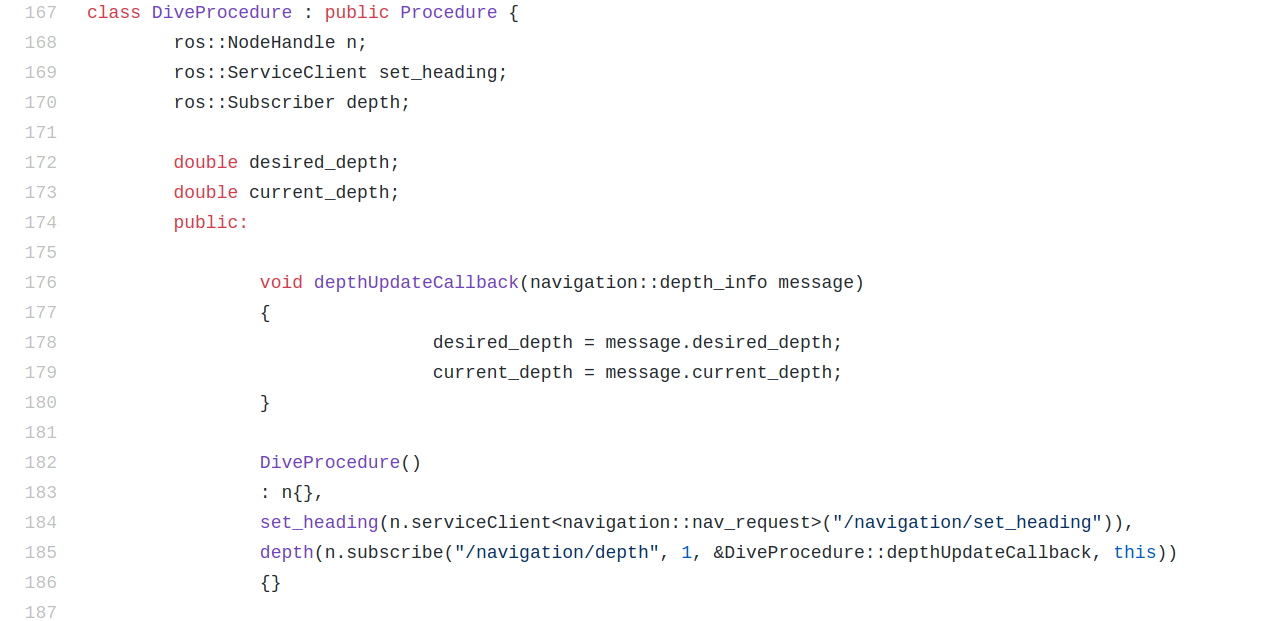
\includegraphics[width=150mm]{Figures/NewProcedureOverhead}
\decoRule
\caption[New Procedure Overhead]{Code segment shows new per-procedure overhead.}
\label{fig:NewProcedureOverhead}
\end{figure}

\section{Successes}

\subsection{Dynamic States}
The dynamic loading of the state machine accomplished its goal of making the
state machine operate in a less complicated way.
The loading of the states dynamically based off a configuration file allowed
functionality to be added and removed easily.
The only downside of this system is that despite the states being loaded in
dynamically the procedures needed to be statically typed and compiled to work
properly this way.
Changes that could make this better would be allowing the procedures to also be
loaded in dynamically through python or some other language.

\subsection{Procedures}

Procedures were a success in that the idea of what they should do was correct.
That is to say that despite the interfaces with accessing resources for and
navigation for moving the AUV the design of the procedures was correct.
Assuming the interfaces worked properly they provided a simple unit for
describing a task within.
Furthermore, assuming the interfaces for resources and navigation were simple
the only remaining issue with writing procedures would be that they cannot be
dynamically loaded.

\subsection{Vision and Navigation Systems}

The separation of duty from the original control system into the vision and
navigation systems allowed for a more maintainable control system.
Though this did lead to issues as mentioned earlier about the complexity of
the systems interfaces.
If the procedures were to be provided with a simple interface to the navigation
system and vision system the procedures would be easier to write and more
effective.
